\documentclass[11pt]{article}

\usepackage[margin=1in]{geometry}
\usepackage[T1]{fontenc}
\usepackage[utf8]{inputenc}
\usepackage{lmodern}
\usepackage{graphicx}
\usepackage{booktabs}
\usepackage{hyperref}
\usepackage{xcolor}
\usepackage{caption}
\usepackage{subcaption}
\usepackage{float}

\newcommand{\PaperTitle}{TRM for MCP: Context for Free}
\newcommand{\TriviaQuestionCount}{13}
\newcommand{\TriviaClosedSafe}{0.769}
\newcommand{\TriviaStuffedSafe}{1.000}
\newcommand{\TriviaMcpSafe}{1.000}
\newcommand{\TriviaRouteSafe}{0.308}
\newcommand{\TriviaPromptSafe}{183.3}
\newcommand{\TriviaRetrievedSafe}{46.7}
\newcommand{\StoryworldToolAcc}{1.000}
\newcommand{\StoryworldSmokeQueries}{3}
\newcommand{\StoryworldEventCount}{32}
\newcommand{\StoryworldMeanPrompt}{2379.8}
\newcommand{\StoryworldMeanLatency}{36.5}
\newcommand{\StoryworldFallbackRate}{0.281}
\newcommand{\ArtifactFranceGermanyKB}{75.0}
\newcommand{\ArtifactHiveGlamKB}{112.4}
\newcommand{\ArtifactShadowBioKB}{113.6}


\hypersetup{
  colorlinks=true,
  linkcolor=blue!50!black,
  urlcolor=blue!50!black,
  citecolor=blue!50!black
}

\title{\PaperTitle}
\author{Patri Friedman and Codex}
\date{April 17, 2026}

\begin{document}
\maketitle

\begin{abstract}
We study whether a tiny transformer router model (TRM) can turn MCP from a prompt-formatting trick into a real context-extension mechanism for small language models running under hard memory limits. The core claim is operational rather than mystical: a 2B model does not need to carry the whole world in its prompt if MCP cards and route policies let it pull only the relevant fragments at answer time. Two environment studies support that claim. In a storyworld pipeline, context-bounded MCP packets let small models operate over outputs far larger than the active prompt window while preserving structured phase behavior. In a frozen trivia benchmark, the same 2B model on a capped 4-bit path rises from \TriviaClosedSafe{} closed-book accuracy to \TriviaMcpSafe{} with MCP-routed retrieval on \TriviaQuestionCount{} questions, while using \TriviaRetrievedSafe{} retrieved tokens on average. The remaining weakness is route faithfulness: the safe trained adapter still reaches only \TriviaRouteSafe{} route accuracy even when answer accuracy is perfect.
\end{abstract}

\section{Thesis}
The paper's thesis is narrow: MCP acts as an external memory control plane for tiny models, and a TRM can learn enough of that control policy to make bounded retrieval useful under fixed VRAM and context budgets. ``Context for free'' does not mean free compute or free routing tokens. It means the effective world state available to the model can exceed the active prompt window because the model consults structured external cards instead of carrying the full task state inline.

\section{Experimental Setting}
The trivia study uses a Qwen 3.5 2B checkpoint in 4-bit form on a memory-capped path intended for a 4 GB GPU regime. The evaluated frozen slice contains \TriviaQuestionCount{} questions and compares three answer conditions: closed-book, naive stuffed retrieval, and MCP-routed retrieval. We also track explicit route-label fidelity for the MCP condition.

The storyworld study reuses the bounded-context MCP packetization work that previously produced \ArtifactFranceGermanyKB{}, \ArtifactHiveGlamKB{}, and \ArtifactShadowBioKB{} KB storyworld JSON artifacts. We summarize three context-bounded phase-event corpora and the Qwen 3.5 2B MCP smoke run, which reached tool accuracy \StoryworldToolAcc{} on \StoryworldSmokeQueries{} route queries.

\section{Trivia Environment Study}
Figure~\ref{fig:trivia-accuracy} is the key benchmark figure. Across all three trivia runs, MCP retrieval closes most or all of the gap between closed-book answering and stuffed retrieval. The safe capped adapter matches stuffed retrieval at \TriviaMcpSafe{} answer accuracy, but its route accuracy remains only \TriviaRouteSafe{}, which shows that answer correctness and explicit route policy learning are not the same phenomenon.

\begin{figure}[H]
  \centering
  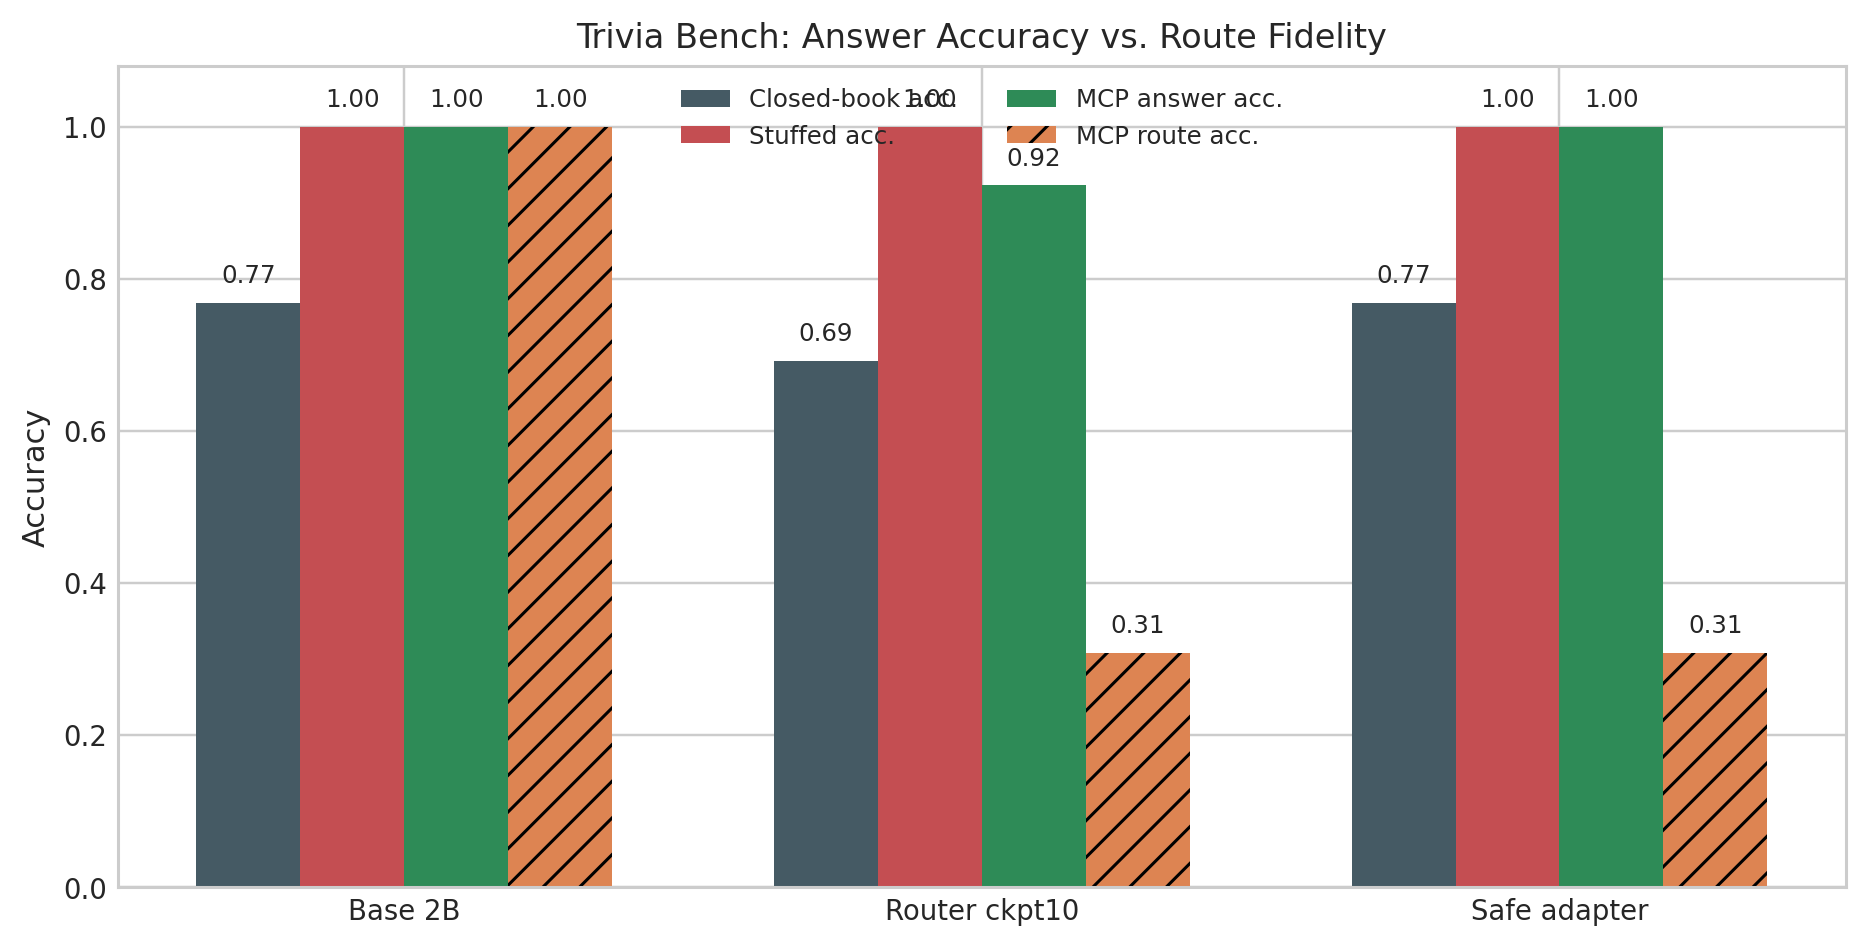
\includegraphics[width=0.92\linewidth]{figures/trivia_accuracy.png}
  \caption{Trivia bench performance across the base 2B run, the interrupted router checkpoint, and the final safe capped adapter. MCP answer accuracy saturates on the frozen slice, but route fidelity lags behind.}
  \label{fig:trivia-accuracy}
\end{figure}

Figure~\ref{fig:trivia-hists} shows the token and latency distributions that matter most for the bench. In the safe capped run, MCP retrieval uses less evidence than the stuffed baseline while keeping answer prompts materially smaller than a naive full-stuffing path. This is the practical point of the setup: the model does not become smarter in closed-book mode, but the retrieval interface lets it spend its narrow context window more selectively.

\begin{figure}[H]
  \centering
  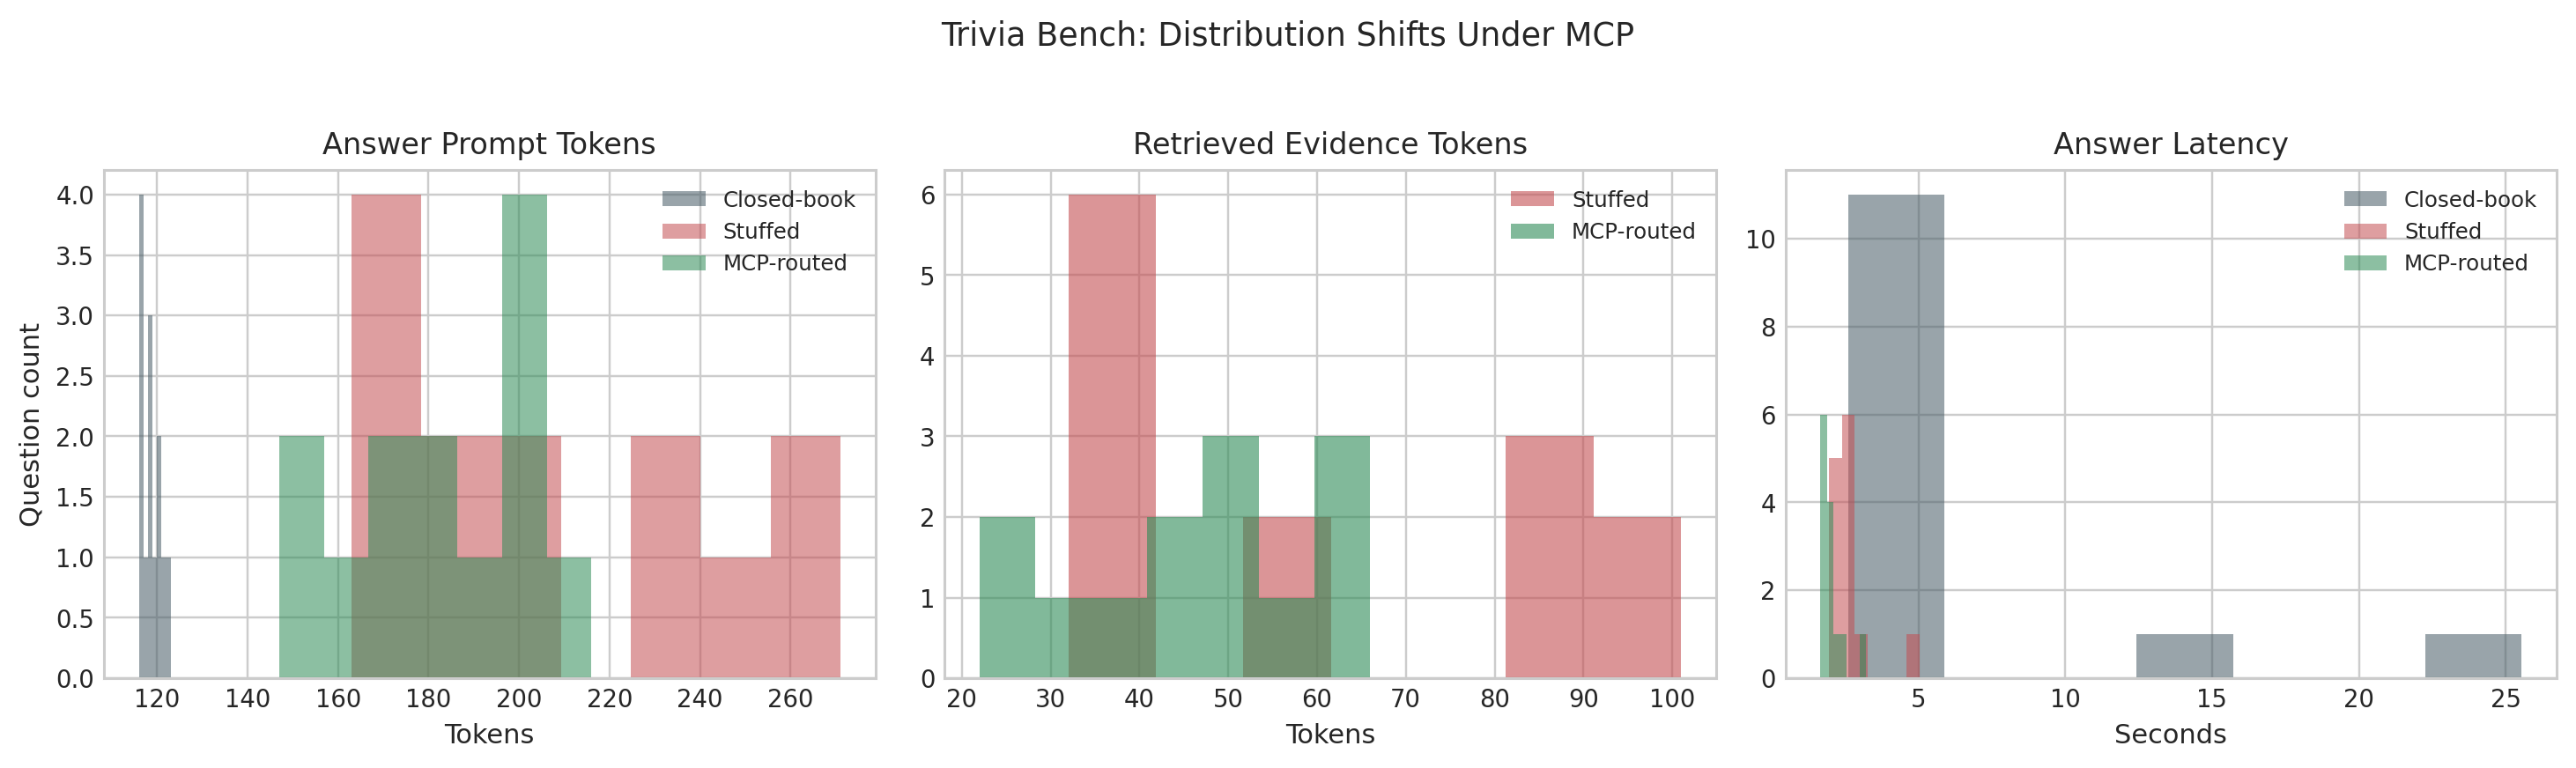
\includegraphics[width=\linewidth]{figures/trivia_histograms.png}
  \caption{Per-question distributions from the safe capped trivia run. MCP reduces retrieved evidence size relative to stuffing while preserving perfect answer accuracy on the frozen slice.}
  \label{fig:trivia-hists}
\end{figure}

\begin{table}[H]
  \centering
  \caption{Trivia benchmark summary. ``Route'' refers to exact router action-label agreement, not final answer correctness.}
  \begin{tabular}{lcccccc}
\toprule
Run & Closed & Stuffed & MCP & Route & Avg. answer prompt & Avg. retrieved \\
\midrule
Base 2B & 0.769 & 1.000 & 1.000 & 1.000 & 162.231 & 32.846 \\
Router ckpt10 & 0.692 & 1.000 & 0.923 & 0.308 & 165.692 & 33.846 \\
Safe adapter & 0.769 & 1.000 & 1.000 & 0.308 & 183.308 & 46.692 \\
\bottomrule
\end{tabular}

\end{table}

\section{Storyworld Environment Study}
The storyworld side of the paper is not a QA benchmark. It is an environment study showing that small models with bounded MCP packets can sustain structured multi-phase generation while producing artifacts that exceed the active prompt window by a large margin. Across \StoryworldEventCount{} recorded phase events, the mean prompt budget usage was \StoryworldMeanPrompt{} tokens and mean phase latency was \StoryworldMeanLatency{} seconds, with aggregate fallback rate \StoryworldFallbackRate{}.

\begin{figure}[H]
  \centering
  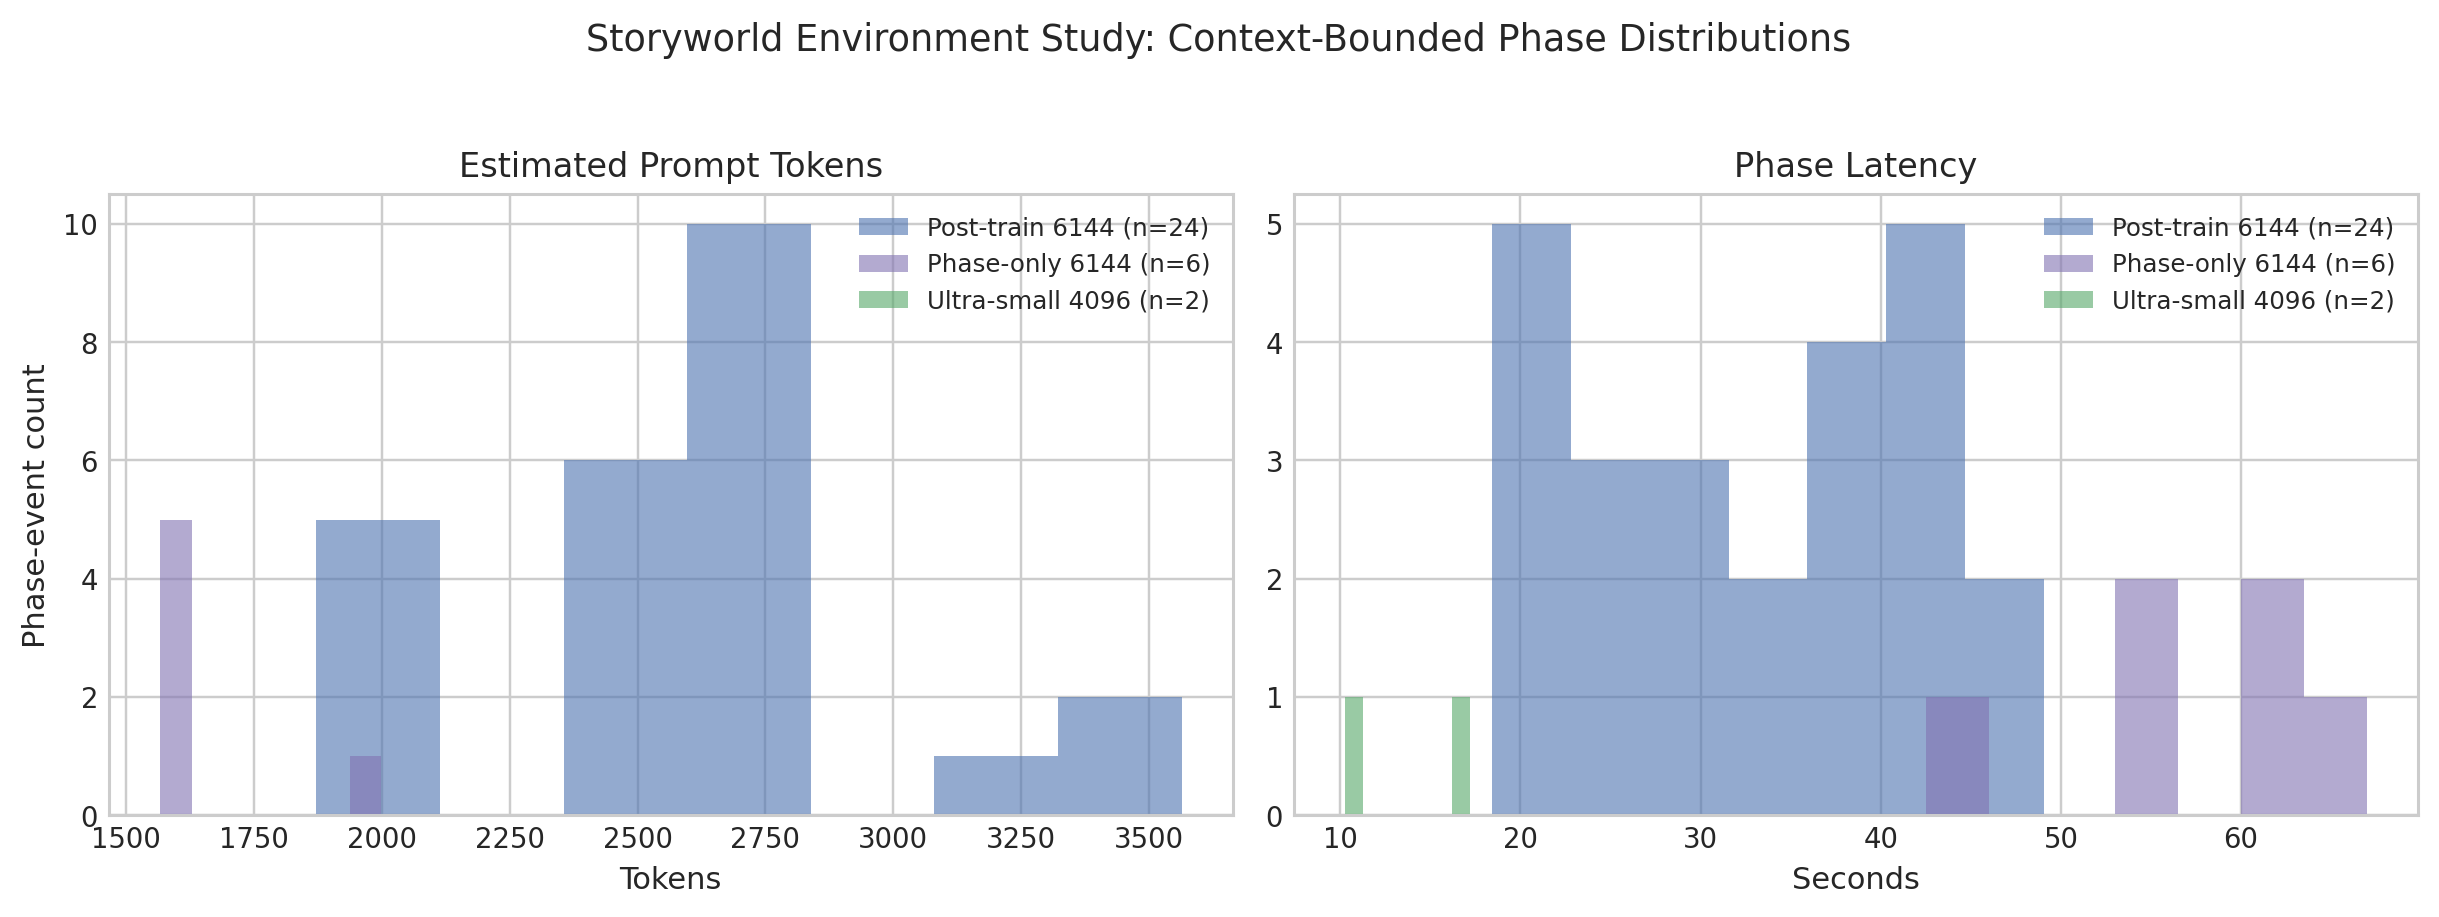
\includegraphics[width=\linewidth]{figures/storyworld_histograms.png}
  \caption{Prompt-token and latency histograms over the storyworld phase-event corpora. The runs cover both 4096-token and 6144-token context budgets.}
  \label{fig:storyworld-hists}
\end{figure}

\begin{figure}[H]
  \centering
  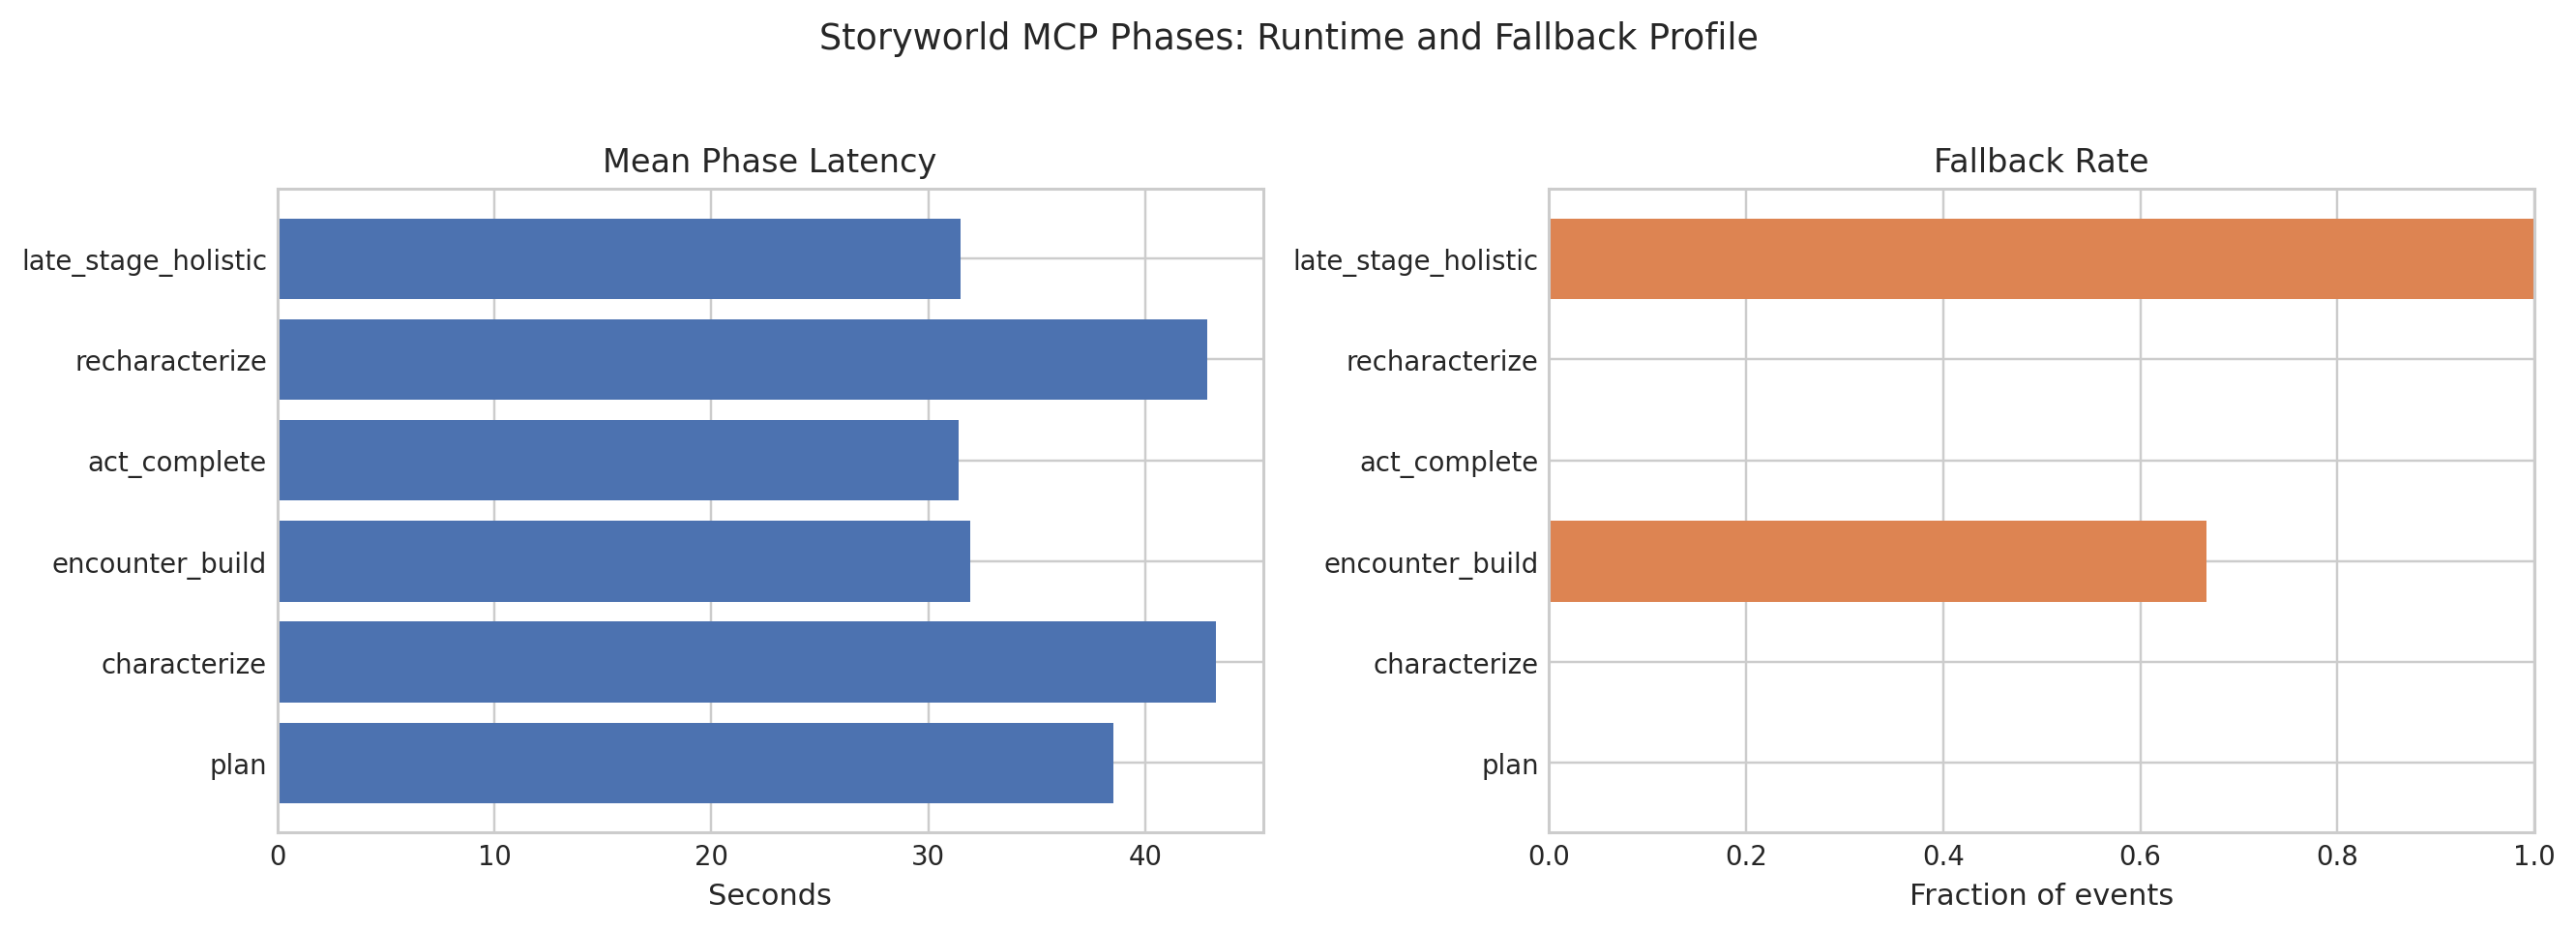
\includegraphics[width=\linewidth]{figures/storyworld_phase_breakdown.png}
  \caption{Phase-level runtime profile over the combined storyworld environment runs. Fallback concentrates in the generation-heavy phases rather than in planning or characterization.}
  \label{fig:storyworld-phase}
\end{figure}

\begin{figure}[H]
  \centering
  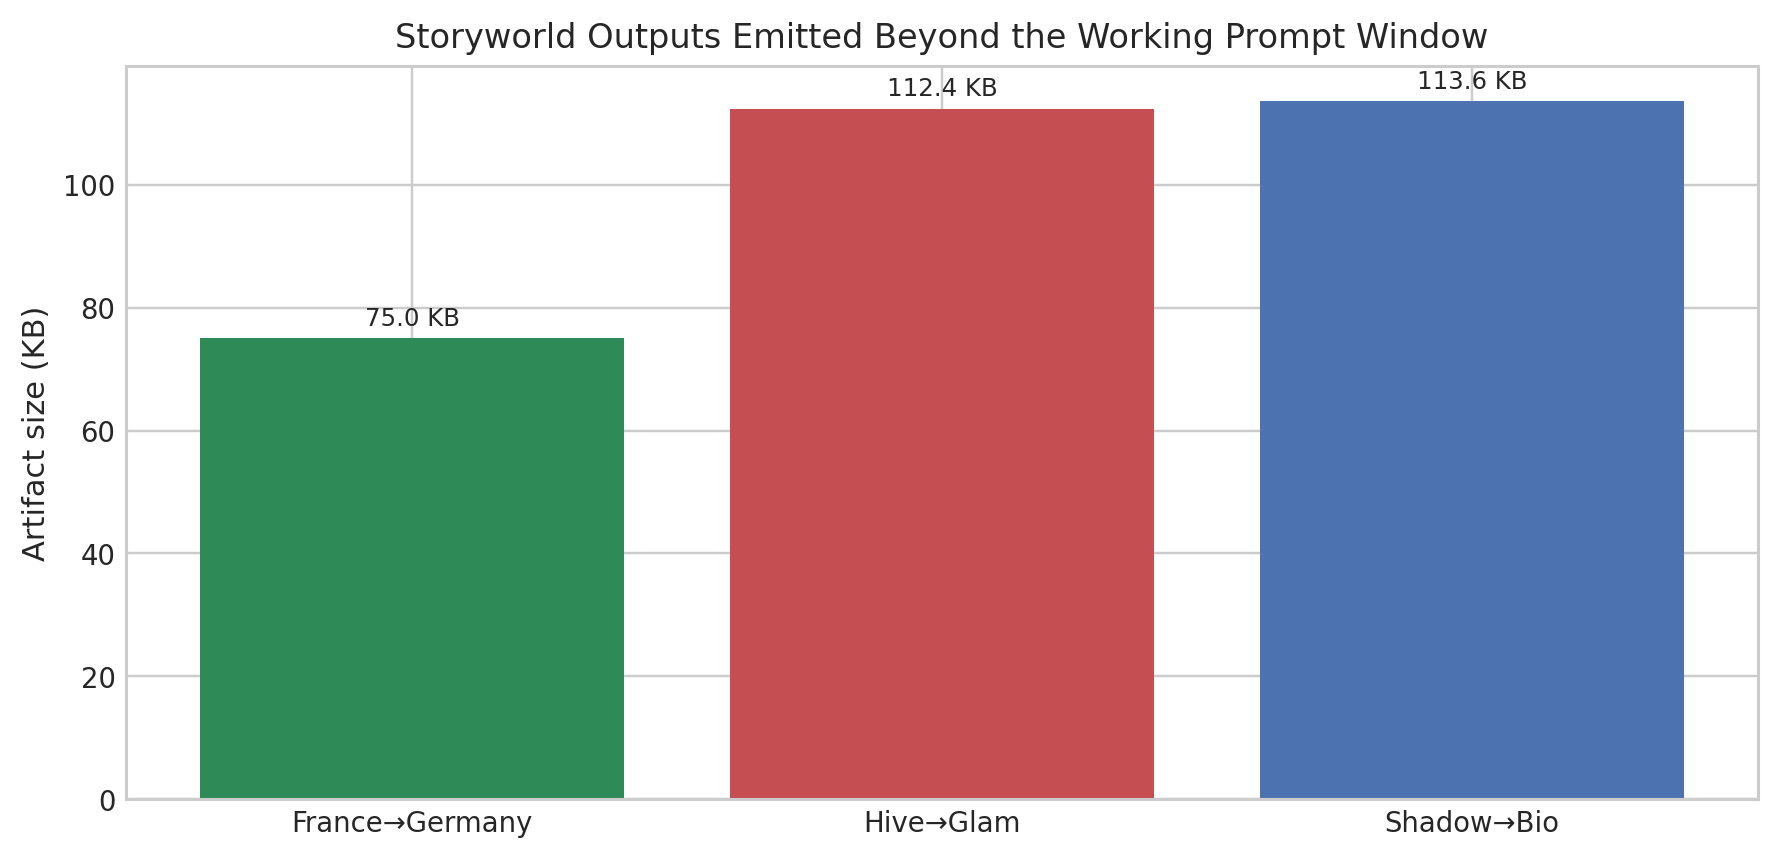
\includegraphics[width=0.82\linewidth]{figures/storyworld_artifacts.png}
  \caption{Representative storyworld artifacts generated in the bounded-context pipeline. The output files are much larger than the working prompt window that produced them.}
  \label{fig:storyworld-artifacts}
\end{figure}

\begin{table}[H]
  \centering
  \caption{Storyworld environment summary from the selected bounded-context runs.}
  \begin{tabular}{lccccc}
\toprule
Run & Context budget & Events & Mean prompt & Mean latency (s) & Fallbacks \\
\midrule
Post-train 6144 & 6144 & 24 & 2549.9 & 33.28 & 7 \\
Phase-only 6144 & 6144 & 6 & 1638.2 & 56.98 & 1 \\
Ultra-small 4096 & 4096 & 2 & 2563.0 & 13.74 & 1 \\
\bottomrule
\end{tabular}

\end{table}

\section{Interpretation}
The combined picture is stronger than either study alone. The storyworld runs show that MCP packetization can externalize large structured state for a tiny model under 4 GB-class constraints. The trivia bench then turns that design into a measurable capability result: the same 2B model that is imperfect closed-book can become perfect on the frozen slice once MCP hands it the right evidence. That is already sufficient for a systems-style paper claim.

The weak point is equally clear. The router has not yet learned a faithful explicit policy. The safe adapter reaches perfect answer accuracy on the frozen trivia slice, but only \TriviaRouteSafe{} route accuracy. That means some answer gains may come from useful but policy-divergent evidence selection rather than clean imitation of the intended MCP routing program.

\section{Next Work}
The next paper-grade step is to harden the trivia bench into a broader suite and then train the TRM directly against the richer MCP index abstraction rather than just the current label space. That would let the paper ask the more interesting question: can a tiny router learn when to query aliases, entity cards, relation cards, or control actions with the same kind of bounded-context discipline already demonstrated in the storyworld pipeline?

\end{document}
